\part{Analyse acoustique du théâtre d'Orange}
\label{part3}

\chapter*{Introduction}
	\addcontentsline{toc}{chapter}{Introduction}
	
%\section{Interface utilisateur} \label{sect_add-on}

La force de ce développement logiciel est que l'utilisateur n'a pas besoin d'effectuer de manipulations complexes pour obtenir les résultats de calcul d'acoustique de salle. Il pourra travailler directement sur son maillage dans le logiciel \gls{cao} et lancer le calcul. Blender permet de développer des scripts en Python qui peuvent par la suite être installés sous forme de \textit{add-on}. L'interface homme-machine de Blender est donc complètement modulable et personnalisable. Le add-on développé dans la cadre de ce projet possède quelques boutons. En utilisant le bouton "Run", Blender transforme les faces des objets sélectionnés en triangle et les exporte au format \gls{obj} (dans le répertoire où se trouve l'exécutable créé en C++). Dans le fichier de maillage, chaque objet est différencié par un en-tête comprenant son nom. S'en suit les coordonnées de l'ensemble de ses sommets (ou vertices), de ses textures et de ses normales. Ensuite sont regroupées par matériaux, les faces par combinaison de trois vertices, d'une texture et d'une normale. Un vecteur de sommets et un vecteur de normales sont remplis face par face en conservant le même ordre. Ces deux vecteurs stockent ainsi la totalité du maillage. Les textures quant à elles ne nous sont pas utiles. Les coefficients d'absorption des matériaux sont aussi assemblés dans un vecteur en les classant face par face en respectant l'ordre établi précédemment.

\begin{figureth}
	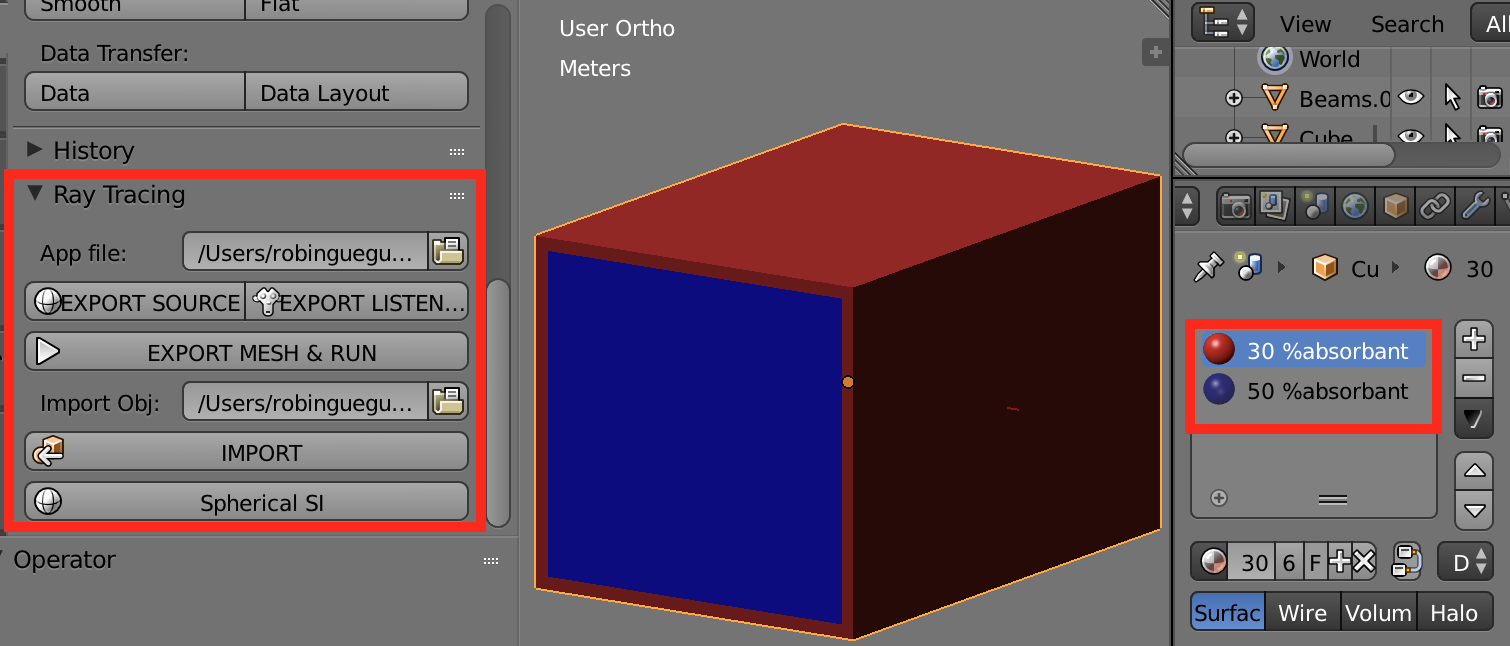
\includegraphics[width=\linewidth]{images/add-on}
	\caption{Add-on Blender et assignation des matériaux}
\end{figureth}

Par défaut, une source et un récepteur sont positionnés au point [0, 0, 0]. Le rayon de mesure du récepteur est de 1m. Cependant, l'utilisateur pourra changer ces paramètres en créant des objets source et récepteur dans Blender. Pour être reconnus et discriminés du maillage, ces objets doivent respectivement comporter les mots "\textit{source}" et "\textit{listener}" dans leur nom. L'algorithme déterminera alors le centre des objets sources et des récepteurs en calculant la moyenne des coordonnées des sommets. Le rayon de mesure du récepteur correspond au rayon de la sphère circonscrite à l'objet "\textit{listener}". Notons qu'il est possible de placer plusieurs sources. L'ensemble des calculs se réaliseront séquentiellement pour une source après l'autre. Un seul récepteur est pris en compte. L'add-on Blender permet de mettre à jour uniquement les informations sur les sources et récepteurs sans avoir besoin de recharger tout le maillage.
Par ailleurs l'utilisateur assignera aux différentes parois un type de matériau en faisant apparaitre dans son nom la référence du matériau issue de la base de donnée Odéon (voir section \ref{sect_lectMat}). La température et pression sont également paramètrables.
A completer ...

	
			
	
\chapter{Configuration initiale}
	\citationChap{
	Les idées sont comme des êtres vivants. Elles naissent, elles croissent, elles prolifèrent, elles sont confrontées à d'autres idées et elles finissent par mourir.
	}{Bernard Werber}
	\minitoc
	\newpage
	
	\section{Configuration du maillage}
	\section{Les matériaux}
	\section{RIR du théâtre d'Orange}
		
	\chapter{Test de configurations}
		\citationChap{
	Don't stop me now \\
	I'm having such a good time, I'm having a ball \\
	Don't stop me now\\
	If you wanna have a good time just give me a call \\
	Don't stop me now\\
	'Cause I'm having a good time \\
	Don't stop me now \\
	Yes I'm havin' a good time \\
	I don't want to stop at all
		}{Queen}
		\minitoc
		\newpage
	
		\section{Position des spectateurs}
			\subsection{Devant}
			\subsection{Derrière}
			\subsection{Jardin}
			\subsection{Cours}
		\section{Présence de spectateurs}
		\section{Présence de velum}
		\section{Forme et matériaux du toit}
		
		\newpage

	\chapter{Comparaison avec d'autres théâtres antiques}
		\citationChap{
		Si on veut connaitre un peuple, il faut écouter sa musique
		}{Platon}
		\minitoc
		\newpage
	
	\chapter*{Conclusion}
	\addcontentsline{toc}{chapter}{Conclusion}
	
		\newpage
		
% Biblio
 \bibliographystyle{francaissc}
 \bibliography{Part3/Biblio}
\addcontentsline{toc}{chapter}{Références}
